%\documentclass{beamer}

\documentclass[handout]{beamer}
\usepackage{pgfpages}
\pgfpagesuselayout{2 on 1}[a4paper,border shrink=5mm]
%\setbeameroption{show notes}

\usepackage{siunitx}
\usepackage{graphicx}

\usetheme{Montpellier}

\title{Effect of low-rise building geometry on tornado-induced loads}
\author{140926~WANG Yong}
\institute{Southeast University}
\date{\today}

\begin{document}

\begin{frame}
	\titlepage
\end{frame}

\section*{Outline}
\begin{frame}
	\tableofcontents
\end{frame}

\section{Introduction}

\begin{frame}
    \frametitle{Challenges to quantify  tornado-induced loads:}
    \begin{itemize}
    	\item<1-> Lack of research facilities capable of determining tornado-induced loads (pressures, forces, etc.)
    	\item<2-> Absence of full-scale data
    	\item<3-> Lack of interest in tornado-resistant design
    		\note[item]<1> {Because the tornado is occasional and has destructive capacity. }
    		\note[item]<2> {This is the direct result of the first limitation. Because of this, we can hardly understand the real structure of the tornado wind field.}
    		\note[item]<3> {Because people used to believe that tornado resistent design is impossible.}
    \end{itemize}
\end{frame}


\begin{frame}
    \frametitle{How to overcome these challenges:}
    \begin{itemize}
    	\item<1-> Iowa State University (ISU) tornado simulator
    		\note[item]<1> {This tornado simulator is capable of creating a simulated tornado, which can travel relative to a building model.}
    	\item<2-> Full-scale data from several recent tornados
    		\note[item]<2> {There is a research team named VORTEX, and it uses Doppler Radar On Wheels to chase the tornado.}
    	\item<3-> Pressures obtained form  the ISU simulator are verified
    	 	\note[item]<3> {Input the pressures into the FEA model, the real damage of full-scale building can be replicated.}
    \end{itemize}
\end{frame}


\section{Description of simulated tornado}
\subsection{Maximum horizonal wind speed}

\begin{frame}
	\frametitle{Maximum horizontal wind speed}
	\begin{description}
		\item[Fact 1:  ]<1-> Around 90\% of all tornados are rated F2 or less
			\note[item]<1> {It's Fujita scale to measure the intensity of tornado.}
		\item[Fact 2: ]<2-> Maximum velocity of F2 tornado is \alert{\SI{74}{m/s}}
		\item[Fact 3: ]<3-> Design wind speed ranges from \alert{\SI{63}{m/s}} to \alert{\SI{80}{m/s}} (ASCE 7-10, 2010)
			\note[item]<3> {We can find that the Maximum vvelocity of F2 tornado is the same order of magnitude with the design wind. So it is possible for tornado resistent design.}
		\item[Fact 4: ]<4-> Maximum horizonal velocity of the tornado generated by ISU Simulator is \alert{\SI{11.7}{m/s}}
	\end{description}
	\begin{block}<5->{Choose target full-scale wind speed to be \alert{\SI{74}{m/s}}}
			 Velocity scale $\lambda_v=11.7/74=1/6.3$
	\end{block} 
\end{frame}

\begin{frame}
	\frametitle{Contour plot of normalized tangential velocity}
		\note{This is the contour plot of normalized tangential velocity of ISU simulated tornado. $r_c$ is core radius, it will be defined later.}
	\begin{figure}
	\centering
	\caption{Contour plot of tangential velocity magnitudes normalized with respect to the maximum tangential velocity}
	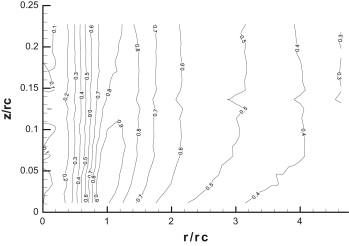
\includegraphics{./fig/1.jpg}
	\end{figure}

\end{frame}

\subsection{Tornado vortex diameter}

\begin{frame}
	\frametitle{Tornado vortex diameter}
	\begin{definition}
	 	\alert{Radius of the core $r_c$}: radius of the maximum wind near the ground
	\end{definition}
		\note{It is found that the damage to building may occur withein a diameter, so the radius of the core is important.}
	\begin{description}
		\item[Fact 1: ]<2-> $r_c$ of F2 tornado is between \alert{\SI{45}{} to \SI{225}{m}}
		\item[Fact 2: ]<3-> $r_c$ of simulated tornado is \alert{\SI{0.56}{m}}
	\end{description}
	\begin{block}<4->{Choose $r_c$ of target full-scale tornado to be \alert{\SI{56}{m}}}
		   Length scale is $1:100$ 
	\end{block} 
\end{frame}

\subsection{Swirl ratio}

\begin{frame}
	\frametitle{Swirl ratio: definition}
	\begin{definition}
		\alert{Swirl ratio $S$}: 
		$$ S = \frac{\pi V_{\theta\mathrm{max}} r_c^2}{Q}$$
		\begin{description}
			\item[$r_c$: ] core radius
			\item[$V_{\theta\mathrm{max}}$: ] maximum tangential wind speed
			\item[$Q$: ] inflow rate of the vortex measured at $r=r_c$
		\end{description}
	\end{definition}
		\note{Swirl ratio is an important parameter, because vortex structure is related to the swirl ratio.}
\end{frame}

\begin{frame}
	\frametitle{How to choose swirl ratio}
		\begin{description}
			\item[Fact 1: ] <2-> Data from full-scale tornados indicates \alert{$S\geqslant2.0$}
			\item[Fact 2: ]<3-> Best fit of full-scale data with numerical simulation when \alert{$S\geqslant2.0$}
		\end{description}
		\begin{block}<4->{Choose the swirl ratio $S$  to be \alert{\num{2.6}} }
			
		\end{block}
			\note{The ISU tornado simulator has vane to generate shear wind. Change the vane angle, the swirl ratio can be varied.}
\end{frame}


\section{Model description, instruments,  conventions}
\subsection{Building models}
\begin{frame}
	\frametitle{Building models}
	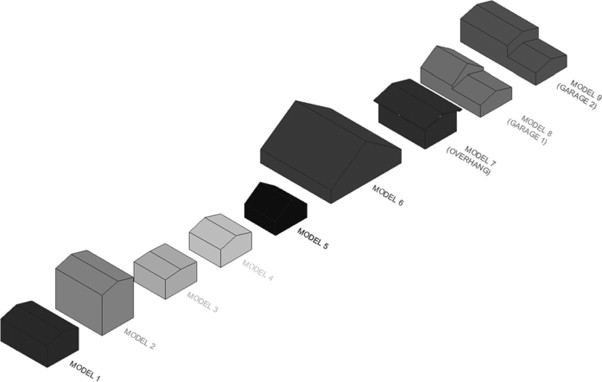
\includegraphics[width=0.8\textwidth]{./fig/2.jpg}
	\note{These nine building models have varying roof pitched, eave heights, aspect ratio and so on. We can see the true dimension in this page.}
\end{frame}

\begin{frame}
	\frametitle{Model dimensions}
	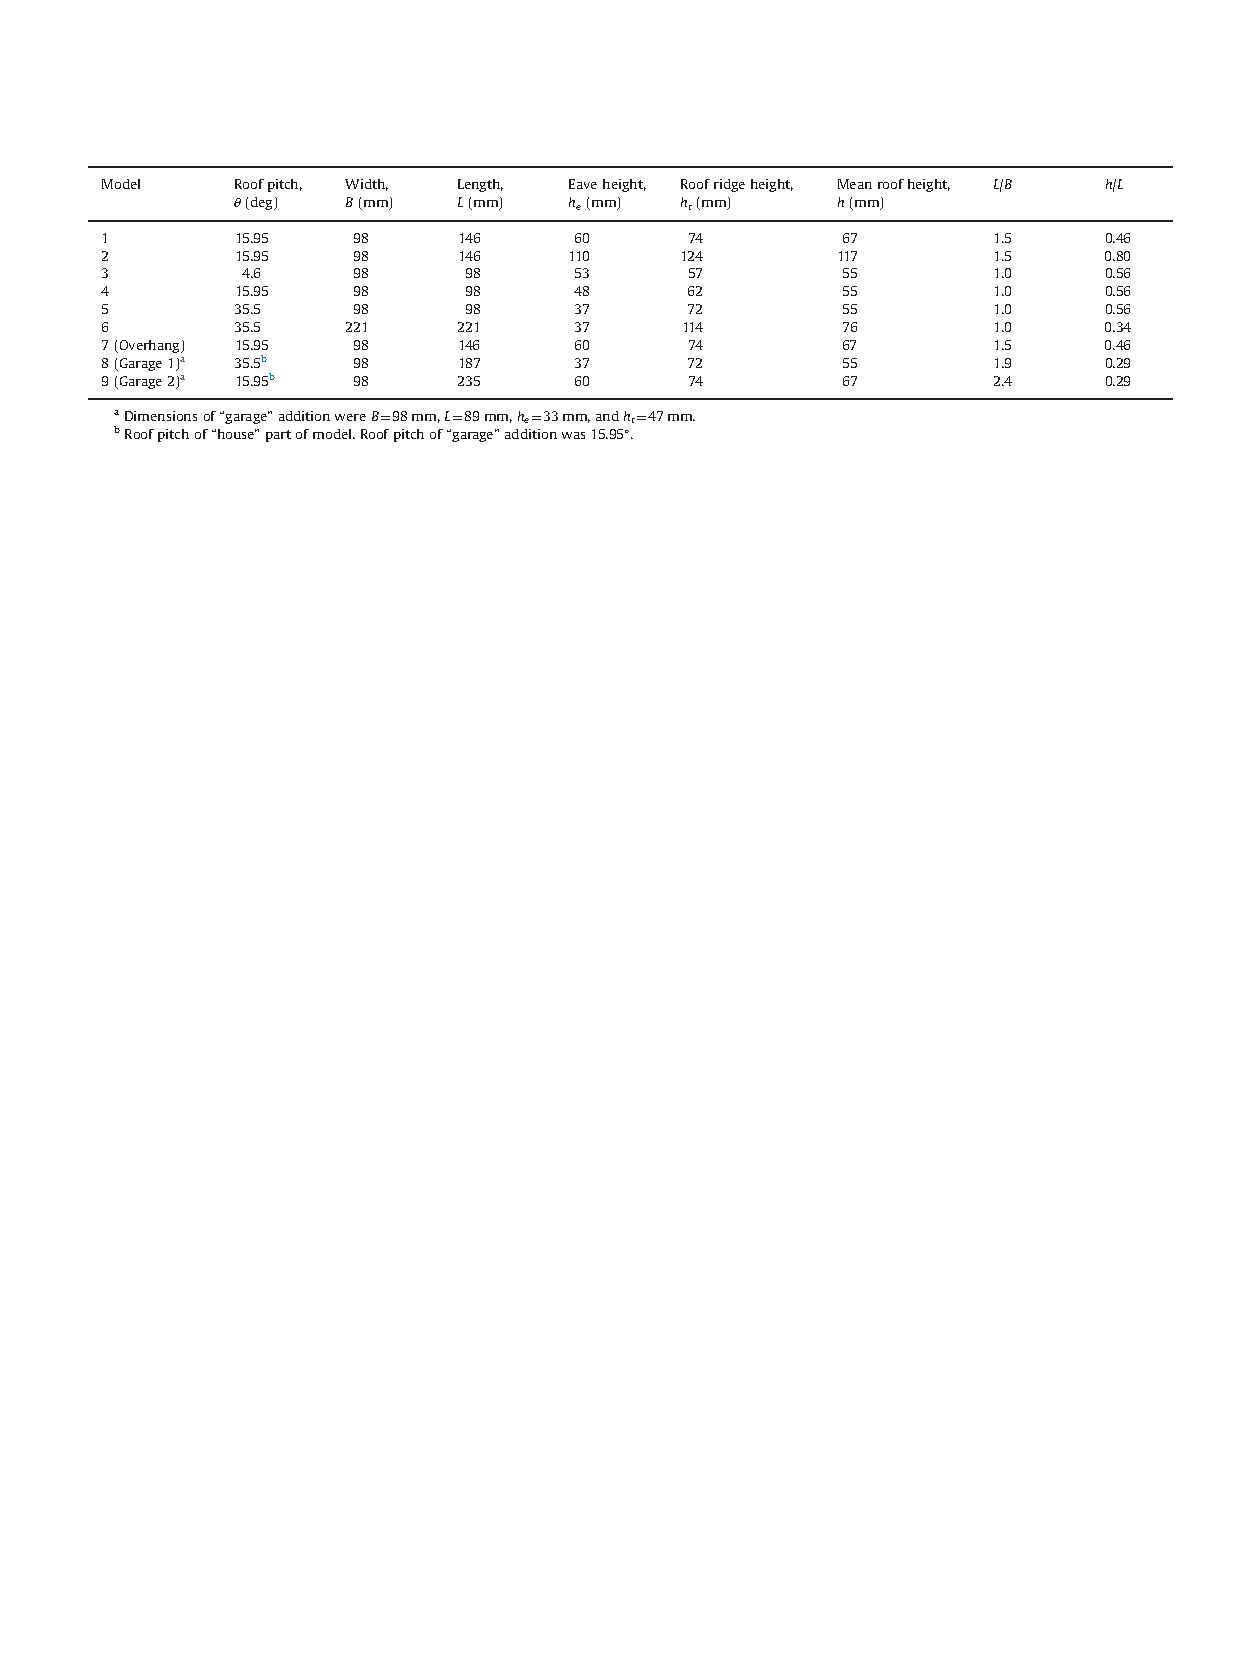
\includegraphics[width=\textwidth]{./fig/model_dimension.pdf}
		\note{This page lists the dimensions of the building models, which is real scaled version of the common full-scale buildings.}
\end{frame}

\subsection{Instrumentation}
\begin{frame}
	\frametitle{Wind velocity measurement: Cobra probe}
	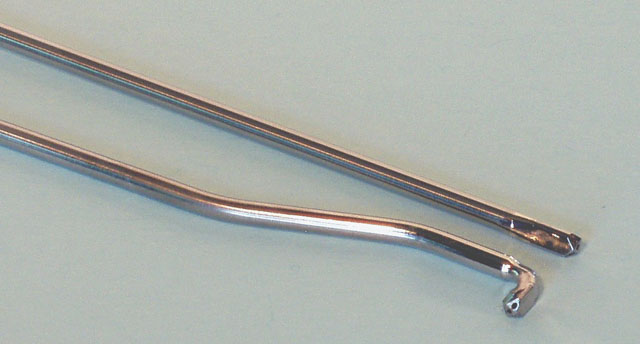
\includegraphics[width=0.6\textwidth]{./fig/speed_measure.jpg}
	\begin{block}<2->{Measurement points}
	horizontally spaced at \SI{50.8}{mm}
	
	vertically spaced at \SI{6.35}{mm}
	\end{block}
\end{frame}

\begin{frame}
	\frametitle{Pressure measurement: ZOC33/64Px pressure transducer}
	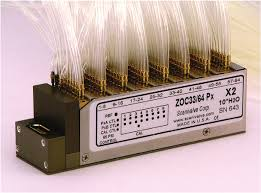
\includegraphics[width=0.6\textwidth]{./fig/pressure_measure.jpg}
		\begin{block}<2->{Measurement frequency: \SI{390}{Hz}}
		
		\end{block}
\end{frame}

\subsection{Procedure and conventions}
\begin{frame}
	\frametitle{Procedure}
	\begin{itemize}
		\item<1-> For each test case the pressure were recorded 10 times
		\item<2-> Calculate the peak pressure as the average of the peak pressures from each of the 10 runs
		\item<3> Change the BOA from \ang{0} to \ang{90} with a step size of \ang{15}
	\end{itemize}
	\begin{definition}<3>
		\alert{BOA}: the orientation of the building with respect to the direction of translation of the tornado
	\end{definition}
\end{frame}

\begin{frame}
	\frametitle{BOA \& Areas used to compute force coefficients}
	\begin{figure}
	\centering
	\caption{Building orientation angle (BOA) with respect to the tornado translation axis (X) and areas ($S_v$, $S_z$) used to normalize force coefficients}
		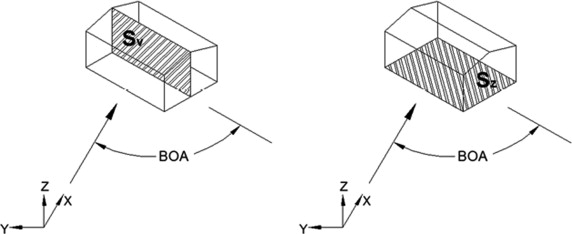
\includegraphics[width=\textwidth]{./fig/3.jpg}
	\end{figure}
	
	
\end{frame}

\begin{frame}
	\frametitle{Calculation of force coefficients}
		\note{The equations used to calculate the force coefficients are given as the following equations.}
	\begin{equation}
		C_{Fx}=\frac{F_x}{(1/2)\rho V_H^2 S_v}
	\end{equation}
	
	\begin{equation}
		C_{Fy}=\frac{F_y}{(1/2)\rho V_H^2 S_v}
	\end{equation}
	
	\begin{equation}
		C_{Fz}=\frac{F_z}{(1/2)\rho V_H^2 S_z}
	\end{equation}
	
	\begin{equation}
		C_{Fxy}=\sqrt{C_{Fx}^2+C_{Fy}^2}
	\end{equation}
\end{frame}

\section{Results}
\subsection{The effect of eave height}
\begin{frame}
	\frametitle{The effect of eave height: Models}
	\begin{description}
		\item[Fact 1: ]<1-> Difference between Model 1 \& 2 was \alert{eave heights $h_e$}
		\item[Fact 2: ]<2-> Model 1:  $h_e=\SI{60}{mm}$ \\
		                                         Model 2:  $h_e=\SI{110}{mm}$
	\end{description}
		\note{We can see that the eave height of Model 2 is almost two times of Model 1.}
\end{frame}

\begin{frame}
	\frametitle{The effect of eave height: Peak pressures}
	\begin{figure}
		\centering
		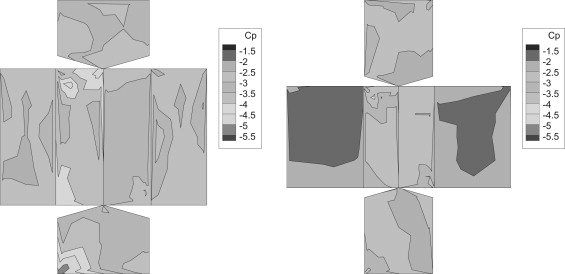
\includegraphics[width=0.8\textwidth]{./fig/4.jpg}
		\caption{Peak pressure contours for Model 1 (left) \& 2 (right), BOA=\ang{30}}
	\end{figure}
	\begin{itemize}
		\item Peak pressure contours of Model 1 \& 2 are similar
		\item Magnitudes of peak pressure: Model 1 $>$ Model 2
	\end{itemize}
		\note{The peak pressures on Model 1 are significantly higher.}
\end{frame}

\begin{frame}
	\frametitle{The effect of eave height: Vertical force coefficient}
	\begin{figure}
		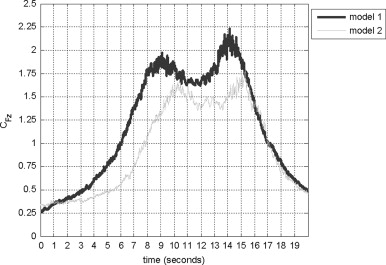
\includegraphics[width=0.8\textwidth]{./fig/5.jpg}
		\caption{$C_{Fz}$ time history for Model 1 \& 2, BOA=\ang{30}}
	\end{figure}
		\note{From this picture, we can easily find that the magnitudes of vertical force coefficient of Model 1 is higher than Model 2. Vertical force coefficient is used to determine the uplift force.}
\end{frame}

\begin{frame}
	\frametitle{The effect of eave height: XY force coefficient}
	\begin{figure}
			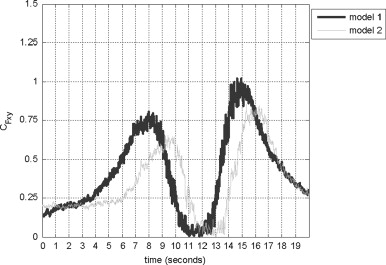
\includegraphics[width=0.8\textwidth]{./fig/6.jpg}
			\caption{$C_{Fxy}$ time history for Models 1 \& 2, BOA=\ang{30}}
		\end{figure}
			\note{From this picture, we can find that Model 1 and Model 2 have similar $C_{Fxy}$ time history.}
\end{frame}

\subsection{The effect of roof pitch}
\begin{frame}
	\frametitle{The effect of roof pitch: Models}
	\begin{description}
		\item[Fact 1: ]<1-> Difference between Model 3, 4  \& 5 was \alert{roof pitch $\theta$}
		\item[Fact 2: ]<2-> Model 3:  $\theta=\ang{4.6}$ \\
		                                         Model 4:  $\theta=\ang{15.95}$ \\
		                                         Model 5:  $\theta=\ang{35.5}$
	\end{description}
		\note{All three models have the same mean roof height, the same plan dimensions, and the same aspect ratios.}
\end{frame}

\begin{frame}
	\frametitle{The effect of roof pitch: Peak pressures}
	\begin{figure}
		\centering
		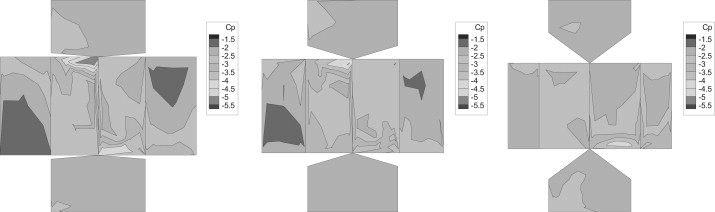
\includegraphics[width=\textwidth]{./fig/7.jpg}
		\caption{Peak pressure contours for Model 3 (left), 4 (center) \& 5 (right), BOA=\ang{45}}
	\end{figure}
	\begin{itemize}
		\item<2-> As $\theta$ $\uparrow$, peak pressure magnitudes for the \alert{roof} $\downarrow$
		\item<3-> As $\theta$ $\uparrow$, peak pressure magnitudes for the \alert{wall} $\uparrow$
			\note[item]<2>{A clear trend occurs in the average peak pressures, as the roof slope increases the peak pressure magnitudes for the roof decrease}
			\note[item]<3> {However, as the roof slope increases the peak pressure magnitudes for the wall increases.}
	\end{itemize}
\end{frame}

\begin{frame}
	\frametitle{The effect of roof pitch: Vertical force coefficient}
	\begin{figure}
		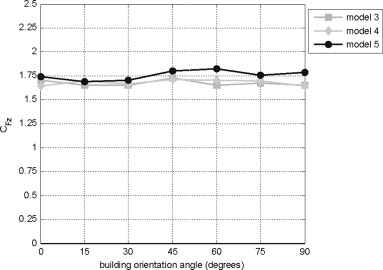
\includegraphics[width=0.8\textwidth]{./fig/8.jpg}
		\caption{$C_{Fz}$ time history for Models 3, 4 \& 5, for each BOA}
	\end{figure}
	\note{We can find that the vertical force coefficient does not change much when the building orientation angle changes.}
\end{frame}

\begin{frame}
	\frametitle{The effect of roof pitch: Vertical force coefficient}
	\begin{figure}
		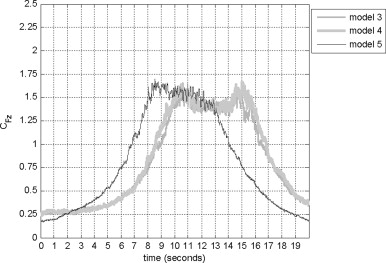
\includegraphics[width=0.8\textwidth]{./fig/9.jpg}
		\caption{$C_{Fz}$ time history for Models 3, 4 \& 5, BOA=\ang{30}}
	\end{figure}
	\note{The vertical force coefficient time history of these three models are almost same with respect to shape and magtitudes as well, the clear difference is in the time when the model experienced the peak value.}
\end{frame}


\section*{The End}
\begin{frame}
\begin{figure}
\centering

\includegraphics[width=\textwidth]{./fig/thank_you.jpg}
\end{figure}

\end{frame}

\end{document}